% Independent native projection probe; not a TikZKit input fixture.
\documentclass{standalone}
\usepackage{pgfplots}
\makeatletter
\let\originalsampledomain\pgfplots@domain@to@foreach
\def\pgfplots@domain@to@foreach#1:#2\relax#3{%
  \originalsampledomain#1:#2\relax{#3}%
  \typeout{SAMPLE #1:#2 (#3): \pgfplotsretval}}
\let\originalfinalscales\pgfplots@scaling@compute@final@scales
\def\pgfplots@scaling@compute@final@scales#1#2#3#4#5{%
  \typeout{SCALE input x=#1 y=#2 inv=#3,#4,#5}%
  \typeout{LIMITS x=\pgfplots@xmin,\pgfplots@xmax; y=\pgfplots@ymin,\pgfplots@ymax; z=\pgfplots@zmin,\pgfplots@zmax}%
  \originalfinalscales{#1}{#2}{#3}{#4}{#5}%
  \typeout{SCALE output xx=\pgfplots@target@unit@scale@xx xy=\pgfplots@target@unit@scale@xy yx=\pgfplots@target@unit@scale@yx yy=\pgfplots@target@unit@scale@yy zx=\pgfplots@target@unit@scale@zx zy=\pgfplots@target@unit@scale@zy}%
}
\newcommand{\extent}{%
  \typeout{RAW LIMITS x=\pgfplots@xmin,\pgfplots@xmax; y=\pgfplots@ymin,\pgfplots@ymax; z=\pgfplots@zmin,\pgfplots@zmax}%
  \coordinate (lo) at (axis description cs:0,0);
  \coordinate (hi) at (axis description cs:1,1);
  \coordinate (b0) at (rel axis cs:0,0,0);
  \coordinate (bx) at (rel axis cs:1,0,0);
  \coordinate (by) at (rel axis cs:0,1,0);
  \coordinate (bz) at (rel axis cs:0,0,1);
}
\newcommand{\report}{%
  \foreach \v in {hi,xl,yl,zl,zscale}{%
    \pgfextractx{\dimen0}{\pgfpointdiff{\pgfpointanchor{lo}{center}}{\pgfpointanchor{\v}{center}}}%
    \pgfextracty{\dimen2}{\pgfpointdiff{\pgfpointanchor{lo}{center}}{\pgfpointanchor{\v}{center}}}%
    \typeout{POINT \v: \the\dimen0,\the\dimen2}}
  \foreach \v in {bx,by,bz}{%
    \pgfextractx{\dimen0}{\pgfpointdiff{\pgfpointanchor{b0}{center}}{\pgfpointanchor{\v}{center}}}%
    \pgfextracty{\dimen2}{\pgfpointdiff{\pgfpointanchor{b0}{center}}{\pgfpointanchor{\v}{center}}}%
    \typeout{BASIS \v: \the\dimen0,\the\dimen2}}
}
\makeatother
\begin{document}
\setbox0=\hbox{$V_{dd}$ in V}\typeout{TEXT X: \the\wd0,\the\ht0,\the\dp0}
\setbox0=\hbox{$f$ in Hz}\typeout{TEXT Y: \the\wd0,\the\ht0,\the\dp0}
\setbox0=\hbox{$P_v$ in mW}\typeout{TEXT Z: \the\wd0,\the\ht0,\the\dp0}
\begin{tikzpicture}
\begin{axis}[width=15cm,view={10}{15},enlargelimits=false,grid=major,
  domain=1.5:6,y domain=0:10^9,ymode=log,samples=46,
  xlabel=$V_{dd}$ in V,ylabel=$f$ in Hz,zlabel=$P_v$ in mW,
  xlabel style={name=xl},ylabel style={name=yl},zlabel style={name=zl},
  every z tick scale label/.append style={name=zscale}]
\addplot3[surf,opacity=.9] {x*x*y};
\extent
\end{axis}
\report
\end{tikzpicture}
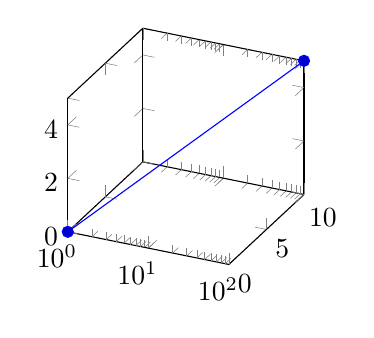
\begin{tikzpicture}
\begin{axis}[scale only axis,width=3cm,height=3cm,xmode=log,
  xmin=1,xmax=100,ymin=0,ymax=10,zmin=0,zmax=5,enlargelimits=false]
\addplot3 coordinates {(1,0,0)(100,10,5)};
\coordinate (lo) at (axis description cs:0,0);
\coordinate (hi) at (axis description cs:1,1);
\end{axis}
\makeatletter
\pgfextractx{\dimen0}{\pgfpointdiff{\pgfpointanchor{lo}{center}}{\pgfpointanchor{hi}{center}}}
\pgfextracty{\dimen2}{\pgfpointdiff{\pgfpointanchor{lo}{center}}{\pgfpointanchor{hi}{center}}}
\typeout{LOG FRAME: \the\dimen0,\the\dimen2}
\makeatother
\end{tikzpicture}
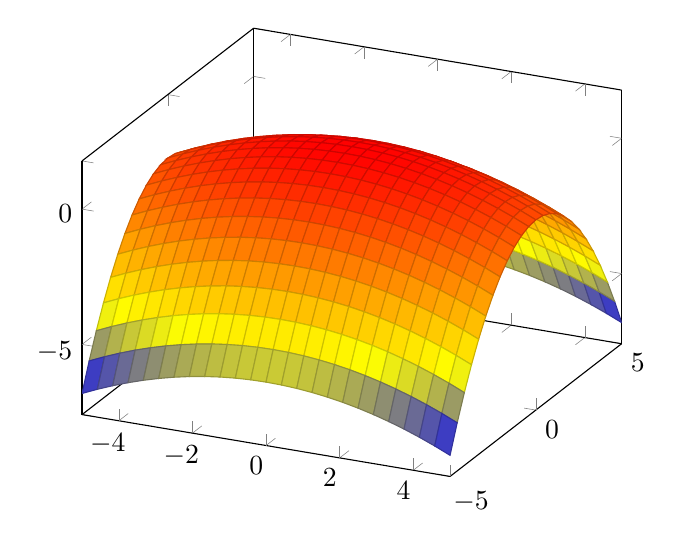
\begin{tikzpicture}
\begin{axis}
\addplot3[surf] {-(x*x/16+y*y/4-1)};
\makeatletter
\typeout{DEFAULT SURVEY: \pgfplots@xmin,\pgfplots@xmax;\pgfplots@ymin,\pgfplots@ymax;\pgfplots@zmin,\pgfplots@zmax}
\makeatother
\end{axis}
\end{tikzpicture}
\end{document}
